%%
%% copyright quintard julien
%% 
%% kaneton
%% 
%% k4-subject.tex
%% 
%% path          /home/mycure/data/research/projects/kaneton/projects/k4
%% 
%% made by mycure
%%         quintard julien   [quinta_j@epita.fr]
%% 
%% started on    Sat Feb 26 15:06:05 2005   mycure
%% last update   Tue May 17 16:00:17 2005   mycure
%%

\documentclass[10pt,a4wide]{article}
\usepackage[english]{babel}
\usepackage{a4wide}
\usepackage[dvips]{graphicx}
\usepackage{graphics}
\usepackage{fancyheadings}
\pagestyle{fancy}

\bibliographystyle{plain}

\lhead{\scriptsize{kaneton project}}
\rhead{k4 subject}
\rfoot{\scriptsize{EPITA System Lab}}

\title{kaneton-4}

\author{Julien Quintard - \small{quinta\_j@epita.fr} \\
        Jean-Pascal Billaud - \small{billau\_j@epita.fr} \\ \\
	\small{last updated by} \\
	Julien Quintard - \small{quinta\_j@epita.fr}}

\date{\today}

\begin{document}
\maketitle

\section{Informations}

\begin{tabular}{p{7cm}l}

Date de rendu: & Lundi 18 Avril 2005 \`a 23h42 \\
Dur\'ee du projet: & 3 semaines \\
Nom du fichier de rendu: & k4.tar.gz \\
Responsable du projet: & Julien Quintard - \small{quinta\_j@epita.fr} \\
                       & Jean-Pascal Billaud - \small{billau\_j@epita.fr} \\
Newsgroups d\'edi\'es: & epita.kaneton, epita.adm.sr \\
Langages: & asm, C \\
Architectures: & Intel 32-bit \\
Nombre de personnes par groupes: & 3 \`a 5

\end{tabular}

\section{Introduction}

\paragraph{}

La gestion de la m\'emoire \'etant disponible, votre kernel est capable
d'allouer de la m\'emoire, que celle-ci soit physique ou bien virtuelle
et si besoin est de la mapp\'ee.

\paragraph{}

Votre kernel dispose de presque toutes les fonctionnalit\'es mises \`a part
une gestion des t\^aches et une gestion des communications inter-processus.

\paragraph{}

Le but de ce projet est donc de fournir une interface pour la gestion
des processus, des threads mais \'egalement le n\'ecessaire pour pouvoir
ordonnancer les fils d'ex\'ecution.

\section{Travail Demand\'e}

\paragraph{}

Dans ce projet nous vous demandons de fournir toutes les interfaces d\'ecrites
dans ce document.

\paragraph{}

De plus l'impl\'ementation de la fonction \textbf{malloc}() sera
obligatoire pour des raisons que vous comprendrez plus loin dans ce document,
plus pr\'ecis\'ement dans la section Ensemble.

\paragraph{}

L'int\'egration d'un fichier de configuration n'est pas obligatoire mais
tout de m\^eme fortement conseill\'e, voir la section Bonus.

\paragraph{}

Une fois toutes les interfaces fournit, votre travail se limitera \`a
tester le bon fonctionnement des t\^aches, des threads, des modules
et de l'ordonnancement.

\section{Nomenclature}

\paragraph{}

Avant toute chose il est important de bien d\'efinir les diff\'erents
termes que nous utiliserons dans ce document. Pour \^etre plus pr\'ecis
nous allons expliciter les termes utilis\'es pour d\'efinir les
diff\'erents types de t\^aches.

\subsection{Module}

\paragraph{}

Un \textbf{module} est une entit\'e particuli\`ere car celle-ci est passive.
En effet un module en soit ne vit pas, ne s'ex\'ecute pas. Un module
est un ex\'ecutable stock\'e en m\'emoire principale plus ou moins longuement
dans le temps. Par exemple les ex\'ecutables des services ou drivers, bref
des t\^aches fondamentales, seront sauvegarder constamment en m\'emoire
principale afin que celles-ci puissent \^etre lanc\'ees et relanc\'ees
tr\`es rapidement et sans aide particuli\`ere.

\subsection{User}

\paragraph{}

Une t\^ache de type \textbf{user} est consid\'er\'ee comme l'entit\'e ayant
les droits les plus faible au niveau syst\`eme. D'un point de vue concret
c'est tout ce que nous nommons ``userland'': les programmes utilisateurs.

\subsection{Service}

\paragraph{}

Un \textbf{service} est une t\^ache qui comme son nom l'indique fournit
un service. En d'autres termes, ce type de t\^ache est appell\'e par
les taches du m\^eme niveau ou inf\'erieur pour effectuer une op\'eration
sp\'ecifique nomm\'ee \textbf{service}.

\subsection{Driver}

\paragraph{}

Un \textbf{driver} est un service particulier dans le sens ou celui-ci
interagit avec le mat\'eriel. Cela ne signifie pas qu'il a des droits
accrus. En effet g\'en\'eralement, le kernel, les drivers et les services
auront concr\`etement les m\^eme droits syst\`emes.

\subsection{Kernel}

\paragraph{}

Pour finir, un \textbf{kernel} est une sorte de super-driver car celui-ci
fournit un service en ayant acc\`es \`a tous les p\'eriph\'eriques mais
\'egalement \`a toutes les structures internes.

\section{Priorit\'e}

\paragraph{}

Les t\^aches peuvent \^etre diff\'erenci\'ees par leurs comportements. Pour
cette raison chaque t\^ache se voit associer un comportement \textbf{behav}.
Ce comportement introduit un interval de priorit\'es pour la t\^ache, celle-ci
pouvant \'evoluer librement dans celui-ci.

\paragraph{}

Comme nous venons de le dire la t\^ache peut donc retoucher sa priorit\'e.
Pour r\'esumer, une t\^ache est toujours associ\'ee \`a: un comportement
\textbf{behav} identifiant le degr\'e de priorit\'e d\'esir\'e et
une priorit\'e courante \textbf{prior} celle-ci \'etant constamment
situ\'ee dans l'interval associ\'e au comportement.

\paragraph{}

Voici les diff\'erents comportements qu'une t\^ache peut prendre:

\paragraph{}

\begin{center}

\begin{tabular}{|p{4cm}|p{4cm}|p{4cm}|}

\hline

\textbf{behaviour}	& \textbf{interval}	& \textbf{default priority} \\

\hline

KERNEL			& [210, 250[		& 230 \\

\hline

REALTIME		& [170, 210[		& 190 \\

\hline

INTERACTIVE		& [130, 170[		& 150 \\

\hline

TIMESHARING		& [50, 130[		& 90 \\

\hline

BACKGROUND		& [10, 50[		& 30 \\

\hline

\end{tabular}

\end{center}

\paragraph{}

Le type \textbf{behav} ne d\'efinit pas la priorit\'e de la t\^ache vis-\`a-vis
de l'ordonnanceur mais bien l'interval dans lequel la t\^ache va pouvoir
\'evoluer.

\paragraph{}

L'ordonnanceur, pour pouvoir correctement d\'ecider du temps \`a attribuer \`a
chaque t\^ache suivant sa priorit\'e, doit garder un certain nombre de
valeurs constamment \`a jour notamment: le nombre de t\^aches actuellement
sur le syst\`eme et le quantum de temps \`a attribuer \`a une t\^ache.
Pour plus d'informations, r\'ef\'erez vous \`a la section Types et plus
pr\'ecis\'ement sur le type \textbf{t\_sched}.

\paragraph{}

Avec ces deux param\`etre l'ordonnanceur sera capable de calculer le temps
processeur \`a attribuer \`a chaque t\^ache en fonction de sa priorit\'e.

\paragraph{}

Bien entendu, comme nous le verrons plus loin dans ce document, il serait
\'egalement n\'ecessaire de calculer le temps processeur de chaque thread
en fonction du nombre de threads dans la t\^ache et du temps processeur
de celle-ci.

\section{Classe}

\paragraph{}

En plus d'avoir un comportement et une priorit\'e courante, chaque
t\^ache se voit attribuer une \textbf{classe} lors de sa cr\'eation.

\paragraph{}

La \textbf{classe} d\'efinit les droits g\'en\'eraux de la t\^ache
vis-\`a-vis du syst\`eme, c'est-\`a-dire les op\'erations autoris\'ees
sur le syst\`eme: le processeur comme les p\'eriph\'eriques.

\paragraph{}

Les diff\'erentes classes de t\^aches sont les suivantes: CLASS\_KERNEL,
CLASS\_DRIVER, CLASS\_SERVICE, CLASS\_USER.

\paragraph{}

Le fait d'appartenir \`a telle ou telle classe ne signifie rien mis \`a
part que dans certaines classes vous pouvez effectuer certaines op\'erations
privil\'egi\'ees.

\paragraph{}

De plus, ces classes permettent de ``trier'' les t\^aches, ceci \'etant
obligatoire pour pouvoir \'etablir un syst\`eme hi\'erarchique.

\subsection{Visualisation}

\paragraph{}

Comme nous venons de le voir, les t\^aches sont toutes distingu\'ees par
rapport \`a leur classe. Gr\^ace \`a cela le syst\`eme peut \^etre divis\'e
en couches, chaque couche ayant des droits diff\'erents vis-\`a-vis du
syst\`eme.

\paragraph{}

Voici une visualisation des couches de classes de \textbf{kaneton}.

\paragraph{}

\begin{figure}[h]
\centerline{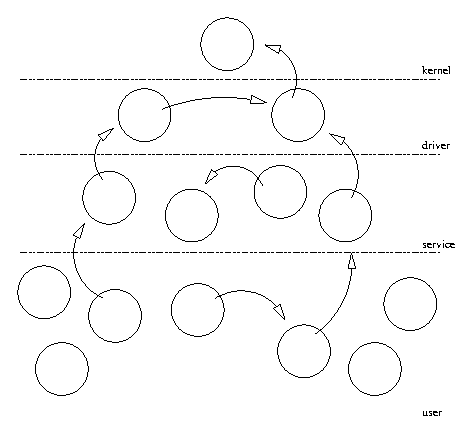
\includegraphics{figures/classes.eps}}
\end{figure}

\paragraph{}

\`A noter que les appels entre les couches sont normalis\'es pour coller
au syst\`eme hi\'erarchique. Les t\^aches peuvent appeller une t\^ache
disposant de privil\`eges sup\'erieurs ou \'egaux aux siens.

\paragraph{}

Ce syst\`eme hi\'erarchique doit absolument \^etre suivi concernant la
demande de service. Par exemple un processus peut demander \`a un service
ou au kernel de faire quelque chose pour lui. En revanche il n'arrivera jamais
que le kernel demande \`a un driver de faire quelque chose pour lui.

\section{Lifetime}

\paragraph{}

Chaque module se voit attribu\'e une dur\'ee de vie nomm\'ee
\textbf{lifetime}.

\paragraph{}

Gr\^ace \`a cette dur\'ee de vie, certains modules resteront charg\'es
en m\'emoire jusqu'\`a l'arr\^et du syst\`eme alors que d'autres se
verront supprim\'es d\`es qu'ils ne seront plus utilis\'es.

\paragraph{}

Bien entendu il est logique de penser que les modules correspondants
au services fondamentaux auront une dur\'ee de vie infinie.

\paragraph{}

Imaginons que le driver IDE crashe \`a cause d'un bug. Il est clair que
les syst\`emes de fichiers ne pourront fonctionner sans driver IDE. Il sera
donc difficile de prendre l'ex\'ecutable du driver IDE sur le syst\`eme
de fichier pour le charger et le relancer puisque toute la gestion
des fichiers sera immobilis\'ee.

\paragraph{}

Gr\^ace au gestionnaire de modules que nous verrons plus loin dans ce document
et au m\'ecanisme de dur\'ee de vie, le driver IDE pourra \^etre relanc\'e sans
difficult\'e car l'ex\'ecutable sera d\'ej\`a charg\'e en m\'emoire.

\paragraph{}

Les diff\'erentes dur\'ees de vie sont: LIFETIME\_INFINITE, LIFETIME\_FINITE

\section{Interfaces}

\paragraph{}

Voici les interfaces \`a suivre pour ce projet.

\subsection{Ensemble}

\paragraph{}

Le gestionnaire d'ensembles f\^ut introduit pour encore une fois simplifer
les autres gestionnaires mais \'egalement les structures de donn\'ees.

\paragraph{}

En effet le gestionnaire d'ensembles s'occupe seul de g\'erer des ensembles
d'objets, de les stocker, de les organiser etc..

\paragraph{}

De ce fait, seul le gestionnaire de m\'emoire physique devra \^etre capable
de g\'erer lui m\^eme sa structure de donn\'ees pour d\'ecrire la m\'emoire
physique du syst\`eme. Au dessus de celui-ci devrait \^etre greff\'e le
gestionnaire de m\'emoire virtuelle mais surtout une fonction
\textbf{malloc}() fournissant une allocation de m\'emoire ad\'equate,
c'est-\`a-dire \textit{\textbf{user-friendly}}.

\paragraph{}

Ensuite le gestionnaire d'ensembles pourrait \'evoluer juste avec ces
services pour fournir un ensemble de fonctionnalit\'es pour stocker
des ensembles de donn\'ees.

\paragraph{}

Une fois le gestionnaire d'ensembles mis en place, tout gestionnaire devrait
y faire appel pour que celui-ci s'occupe de stocker et g\'erer les
donn\'ees.

\paragraph{}

Voici une visualisation du fonctionnement des allocateurs au sein du
kernel.

\paragraph{}

\begin{figure}[h]
\centerline{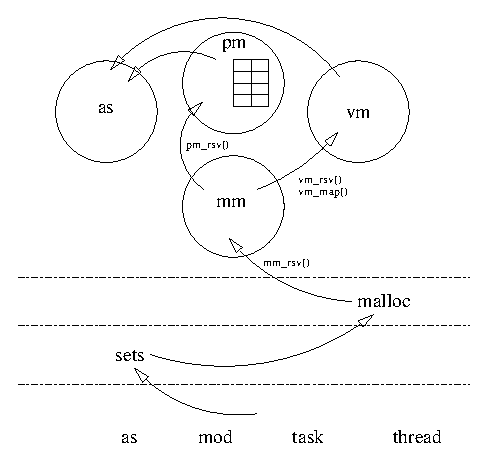
\includegraphics{figures/sets.eps}}
\end{figure}

\paragraph{}

Gr\^ace au gestionnaire d'ensembles, il est extr\^ement simple pour les
autres gestionnaires de g\'erer des donn\'ees car cela n'est pas effectu\'e
en interne mais par le gestionnaire d'ensembles.

\paragraph{}

Le code de chaque gestionnaire devient alors plus simple et plus l\'eger
rassemblant le code g\'erant les structures de donn\'ees dans une seule
unit\'e destin\'ee \`a cet effet: le gestionnaire d'ensembles.

\paragraph{}

Attention, le gestionnaire d'ensembles doit \^etre capable de g\'erer
tout type de donn\'ees, que ce soit des structures complexes type
structures de t\^ache, tout comme des donn\'ees extr\^ement simple
type identifiants.

\paragraph{}

Pour cela plusieurs choix s'offrent \`a vous. Soit vous d\'ecidez que votre
gestionnaire d'ensembles ne comprend pas les types de donn\'ees qu'il g\`ere
mais que les objets de l'ensemble ont besoin d'un identifiant unique et
commun pour pouvoir \^etre retrouv\'es dans l'ensemble.

\paragraph{}

Dans ce cas, la m\'ethode \`a adopter est de normaliser le comportement
d'un objet en obligeant chaque objet \`a fournir un identifiant unique
en d\'ebut d'objet; un identifiant \'etant compris ici comme un nombre
identifiant l'objet de mani\`ere unique dans son ensemble.

\paragraph{}

En l'occurence, il va nous falloir d\'efinir une norme concernant les
identifiants. Cette norme va simplement \^etre constitu\'ee par la
red\'efinition des identifiants du syst\`eme.

\paragraph{}

En effet, nous allons introduire un nouveau type nomm\'e \textbf{t\_id}.
D\'esormais tous les identifiants seront des alias de ce type. Cela implique
quelques modifications dans vos fichiers en-t\^ete. R\'ef\'erez vous
\`a la section Types qui contient la red\'efinition des types des projets
diff\'erents.

\paragraph{}

Ainsi, nous pouvons d\'esormais normaliser le fonctionnement du gestionnaire
d'ensembles: chaque objet contenu dans un ensemble doit obligatoirement
contenir un champ de type \textbf{t\_id} d\'efinissant l'identifiant unique
de l'objet dans son ensemble.

\paragraph{}

Il faut savoir que le gestionnaire d'ensembles est capable de g\'erer
des ensembles de types diverses. Le tableau ci-dessous liste quelque-uns
des types d'ensemble class\'es dans trois cat\'egories: \textbf{sort enabled},
\textbf{sort disabled} et \textbf{manual sort}.

\begin{center}

\begin{tabular}{|p{4cm}|p{4cm}|p{5cm}|}

\hline

\textbf{data structure} & \textbf{type} & \textbf{sort method} \\

\hline

array & SET\_TYPE\_ARRAY & enable - disable - manual \\

\hline

linked list & SET\_TYPE\_LIST & enable - disable - manual \\

\hline

double-linked list & SET\_TYPE\_DLIST & enable - disable - manual \\

\hline

... & ... & ... \\

\hline

\end{tabular}

\end{center}

\paragraph{}

En plus de ces types d'ensembles de base, d'autres types pourront
\^etre impl\'ement\'es en bonus. Pour cela r\'ef\'erez vous \`a la section
Bonus.

\paragraph{}

Voici l'interface \`a suivre dans ce cas.

\paragraph{}

\hspace{1.5cm}int \textbf{set\_init}(void);

\paragraph{}

Cette fonction initialise le gestionnaire d'ensembles.

\paragraph{}

\hspace{1.5cm}int \textbf{set\_rsv}(t\_type \textbf{type},
                                    t\_sort \textbf{sort},
                                    t\_size \textbf{objectsz}, \\
\bigskip
\hspace{3.6cm}                      t\_setsz \textbf{initsz},
                                    t\_setid* \textbf{setid});

\paragraph{}

Cette fonction r\'eserve un ensemble de type \textbf{type}. Chaque objet
de l'ensemble aura une taille de \textbf{objectsz} octets.
L'argument \textbf{initsz} sp\'ecifie la taille initiale de l'ensemble,
en d'autres termes, le nombre d'objets \`a pr\'eallouer. Attention,
\textbf{objectsz} est exprim\'e en octets et \textbf{initsz} est exprim\'e
en nombre d'objets.

\paragraph{}

Certains types d'objets sont laiss\'es en bonus. N\'eanmoins nous attendons
un minimum de types pr\'ed\'efinis comme: SET\_TYPE\_ARRAY, SET\_TYPE\_LIST,
SET\_TYPE\_DLIST, SET\_TYPE\_ANY.

\paragraph{}

Les types sont choisis en fonction de la taille de l'objet, de la rapidit\'e
de recherche d\'esir\'ee, de rapport taille/rapidit\'e etc.. En d'autres
termes, lorsqu'un stockage d'identifiants non-tri\'es sera d\'esir\'e
un tableau sera pr\'ef\'er\'e alors que pour une structure de donn\'ees
tr\`es rapide pour rechercher, par exemple, les structures des threads; une
structure de type arbre sera nettement plus efficace.

\paragraph{}

\`A noter que en fonction du type de l'ensemble certaines op\'erations
d\'ecrites ci-dessous seront autoris\'ees et d'autres interdites.

\paragraph{}

Le type SET\_TYPE\_ANY permet au gestionnaire d'ensembles de choisir
la structure de donn\'ees ad\'equate en fonction de la taille des objets
et du nombre d'objets \`a pr\'eallouer. Il est clair que pour une taille
d'objets de 32-bit, un arbre est surement d\'emesur\'e. En l'occurence
un tableau dyamique est s\^urement le meilleur choix. Rappellons en effet
que le gestionnaire d'ensembles repose sur la fonction \textbf{malloc}()
et donc obligatoirement sur les fonctions qui l'accompagnent comme par
exemple \textbf{realloc}(), \textbf{calloc}(), etc..

\paragraph{}

L'argument \textbf{sort} permet d'indiquer au gestionnaire d'ensembles
comment organiser les objets dans l'ensemble: SET\_SORT\_ENABLE,
indique au gestionnaire de trier les objets tout seul par rapport \`a
l'identifiant, SET\_SORT\_DISABLE indique au gestionnaire d'ensembles
de stocker les objets sans pr\^eter attention \`a l'organisation et
SET\_SORT\_MANUAL indique au gestionnaire d'ensembles que le trie sera
fait manuellement en fonction de param\`etres que le gestionnaire ne
peut pas conna\^itre.

\paragraph{}

\hspace{1.5cm}int \textbf{set\_rel}(t\_setid \textbf{setid});

\paragraph{}

Cette fonction lib\`ere l'ensemble \textbf{setid}.

\paragraph{}

Voyons d\'esormais les fonctions d'int\'eraction avec les ensembles
pr\'ec\'edemment cr\'ees.

\paragraph{}

\hspace{1.5cm}int \textbf{set\_get}(t\_setid \textbf{setid},
                                    t\_id \textbf{id},
                                    t\_iterator* \textbf{iterator});

\paragraph{}

Cette fonction retourne dans \textbf{iterator} l'it\'erateur de l'objet
identifi\'e par \textbf{id}.

\paragraph{}

Attention, cette fonction ne doit pas \^etre utilis\'ee \`a la l\'eg\`ere
car une mauvaise manipulation peut rendre l'ensemble instable. Par exemple,
il ne faut absolument pas modifier l'identifiant de l'objet. Cette remarque
est valable pour toutes les fonctions ci-dessous qui permettent de
retrouver et possiblement modifier un objet.

\paragraph{}

\hspace{1.5cm}int \textbf{set\_head}(t\_setid \textbf{setid},
                                     t\_iterator* \textbf{iterator});

\paragraph{}

Cette fonction retourne dans \textbf{iterator} le premier objet de
l'ensemble \textbf{setid}.

\paragraph{}

\hspace{1.5cm}int \textbf{set\_tail}(t\_setid \textbf{setid},
                                     t\_iterator* \textbf{iterator});

\paragraph{}

Cette fonction retourne dans \textbf{iterator} l'it\'erateur du dernier
\'el\'ement de l'ensemble.

\paragraph{}

\hspace{1.5cm}int \textbf{set\_prev}(t\_setid \textbf{setid},
                                     t\_iterator \textbf{current},
                                     t\_iterator* \textbf{previous});

\paragraph{}

Cette fonction retourne dans \textbf{previous} l'it\'erateur de l'objet
pr\'ec\'edent l'objet \textbf{current}.

\paragraph{}

\hspace{1.5cm}int \textbf{set\_next}(t\_setid \textbf{setid},
                                     t\_iterator \textbf{current},
                                     t\_iterator* \textbf{next});

\paragraph{}

Cette fonction retourne dans \textbf{next} l'it\'erateur de l'objet
succ\'edant l'objet \textbf{current}.

\paragraph{}

\hspace{1.5cm}int \textbf{set\_insert}(t\_setid \textbf{setid},
                                       void* \textbf{object});

\paragraph{}

Cette fonction ajoute l'\'el\'ement \textbf{object} \`a l'ensemble
\textbf{setid}.

\paragraph{}

Les types d'ensembles concern\'es sont: SET\_SORT\_ENABLE et
SET\_SORT\_DISABLE.

\paragraph{}

\hspace{1.5cm}int \textbf{set\_delete}(t\_setid \textbf{setid},
                                       t\_id \textbf{id});

\paragraph{}

Cette fonction s'occupe de d\'etruire l'objet \textbf{id} de l'ensemble
\textbf{setid}.

\paragraph{}

Les types d'ensembles concern\'es sont: SET\_SORT\_ENABLE,
SET\_SORT\_DISABLE et SET\_SORT\_MANUAL.

\paragraph{}

\hspace{1.5cm}int \textbf{set\_insert\_head}(t\_setid \textbf{setid},
                                             void* \textbf{object});

\paragraph{}

Cette fonction ins\`ere l'objet \textbf{object} au d\'ebut de l'ensemble
\textbf{setid}.

\paragraph{}

Les types d'ensembles concern\'es sont: SET\_SORT\_MANUAL.

\paragraph{}

\hspace{1.5cm}int \textbf{set\_insert\_tail}(t\_setid \textbf{setid},
                                             void* \textbf{object});

\paragraph{}

Cette fonction ins\`ere l'objet \textbf{object} \`a la fin de l'ensemble
\textbf{setid}.

\paragraph{}

Les types d'ensembles concern\'es sont: SET\_SORT\_MANUAL.

\paragraph{}

\hspace{1.5cm}int \textbf{set\_insert\_before}(t\_setid \textbf{setid},
                                               t\_id \textbf{id},
                                               void* \textbf{object});

\paragraph{}

Cette fonction ins\`ere l'objet \textbf{object} avant l'objet identifi\'e
par \textbf{id}.

\paragraph{}

Les types d'ensembles concern\'es sont: SET\_SORT\_MANUAL.

\paragraph{}

\hspace{1.5cm}int \textbf{set\_insert\_after}(t\_setid \textbf{setid},
                                              t\_id \textbf{id},
                                              void* \textbf{object});

\paragraph{}

Cette fonction ins\`ere l'objet \textbf{object} apr\`es l'objet identifi\'e
par \textbf{id}.

\paragraph{}

Les types d'ensembles concern\'es sont: SET\_SORT\_MANUAL.

\paragraph{}

\hspace{1.5cm}int \textbf{set\_clean}(void);

\paragraph{}

Cette fonction r\'einitialise le gestionnaire d'ensembles.

\paragraph{}

\`A savoir que le gestionnaire d'ensembles n'accepte aucune collision.
C'est \`a dire que les identifiants dans un ensemble \textit{doivent}
\^etre unique. Si cette r\`egle n'est pas respect\'ee, le gestionnaire
d'ensembles ne peut garantir de bons r\'esultats.

\paragraph{}

De plus, l'utilisateur d'un ensemble doit \^etre conscient du type
de l'ensemble lorsqu'il effectue des op\'erations. En effet ins\'erer
un objet avant un autre lorsque le type de l'ensemble est SET\_TYPE\_ARRAY
et que le nombre d'\'el\'ements de l'ensemble est important n'aura pas les
m\^eme cons\'equences au niveau performances que de le faire dans un
ensemble du type SET\_TYPE\_BTREE par exemple.

\paragraph{}

Il serait int\'eressant de greffer des types au dessus des types de base.
Par exemple il serait int\'eressant de pouvoir cr\'eer facilement et
sans effort des ensembles de type: SET\_TYPE\_STACK, SET\_TYPE\_QUEUE,
SET\_TYPE\_CIRCULAR etc.. car ceux-ci sont tr\`es utile dans un kernel,
pour l'ordonnanceur par exemple.

\paragraph{}

Il vous faudra certainement pour cela d\'efinir une interface suppl\'ementaire.
Libre \`a vous concernant l'\'etablissement de cette interface.

\paragraph{}

Il existe un autre moyen de fournir un service du type gestionnaire d'ensembles
mais d'une mani\`ere beaucoup plus g\'en\'erique en utilisant des
\textbf{templates} en C. Nous ne nous \'etalerons pas sur ce sujet. Pour
de plus amples informations sur ce sujet, r\'ef\'erez vous \`a la
section Bibliographie.

\paragraph{}

L'interface devra \'egalement \^etre constitu\'ee d'une macro pour faciliter
l'exploration d'un ensemble.

\paragraph{}

\hspace{1.5cm}\textbf{SET\_FOREACH}(\_mode\_, \_setid\_, \_iterator\_)

\paragraph{}

Cette macro va parcourir un ensemble en fonction du mode de travers\'ee
\textbf{\_mode\_}: FOREACH\_FORWARD qui va parcourir de la t\^ete vers
la queue et FOREACH\_BACKWARD qui va parcourir de la queue vers la t\^ete.
Bien entendu cette macro utilisera les fonctions: \textbf{set\_head}(),
\textbf{set\_tail}(), \textbf{set\_prev}() et \textbf{set\_next}().
Pour plus d'informations sur la macro, r\'ef\'erez vous \`a la section
Types et plus particuli\`erement au type \textbf{t\_set}.

\paragraph{}

Cette macros est tr\`es simple d'utilisation comme le d\'emontre ce
petit exemple:

\begin{verbatim}
{
  t_iterator    iterator;
  t_setid       setid;

  [...]

  set_rsv([...], &setid);

  set_insert([...]);
  set_insert([...]);
  set_insert([...]);

  SET_FOREACH(FOREACH_FORWARD, setid, &iterator)
    {
      printf(``[object] id:%u addr:0x%x\n'',
             ITERATOR_ID(&iterator),
             ITERATOR_ADDR(&iterator));
    }
}
\end{verbatim}

\subsection{Ordonnanceur}

\paragraph{}

L'interface de l'ordonnanceur est simple mais permet n\'eanmoins la gestion
de priorit\'es sur les tasks comme sur les threads.

\paragraph{}

\`A noter que le gestionnaire de t\^aches, le gestionnaire de threads et
l'ordonnanceur \'evoluent ensemble et modifient tous la structure principale
de l'ordonnanceur pour maintenir l'ordonnancement \`a jour en ce qui
concerne les priorit\'es par exemple.

\paragraph{}

Attention, l'ordonnanceur s'occupe d'ordonnancer des threads et non
des t\^aches. En effet dans \textbf{kaneton}, une t\^ache est consid\'er\'ee
comme un conteneur alors qu'un thread est une entit\'e active.

\paragraph{}

\hspace{1.5cm}int \textbf{sched\_init}(t\_quantum \textbf{quantum});

\paragraph{}

Cette fonction initialise l'ordonnanceur en lui sp\'ecifiant le quantum
de temps par d\'efaut allou\'e \`a chaque processus.

\paragraph{}

Pour b\'en\'eficier d'avantage de temps d'ex\'ecution les processus
peuvent faire \'evoluer leurs priorit\'es suivant leur classe.

\paragraph{}

\hspace{1.5cm}int \textbf{sched\_quantum}(t\_quantum \textbf{quantum});

\paragraph{}

Cette fonction permet de red\'efinir le quantum de temps allou\'e
aux processus.

\paragraph{}

Pour ceux ayant fait un fichier de configuration, il serait int\'eressant
de sp\'ecifier dans ce fichier de configuration le quantum par d\'efaut.

\paragraph{}

\hspace{1.5cm}int \textbf{sched\_yield}(void);

\paragraph{}

Cette fonction permet \`a la t\^ache l'utilisant de redonner la main
\textbf{volontairement} \`a l'ordonnanceur. Cela n'arrive \'evidemment
que lorsque la t\^ache se retrouve bloqu\'ee et que celle-ci pr\'ef\`ere
se d\'egager de son temps processeur car inutilis\'e.

\paragraph{}

\hspace{1.5cm}int \textbf{sched\_next}(t\_thrid* \textbf{thrid});

\paragraph{}

Cette fonction se contente de retourner dans la variable \textbf{thrid}
l'identifiant du prochain thread \`a ex\'ecuter.

\paragraph{}

\hspace{1.5cm}int \textbf{sched\_switch}(t\_thrid \textbf{thrid});

\paragraph{}

Cette fonction effectue le changement de contexte et charge donc le contexte
du thread \textbf{thrid} afin de l'ex\'ecuter.

\paragraph{}

Pensez \`a suivre les indications expliqu\'ees en cours pour pouvoir
ex\'ecuter un changement de contexte sans probl\`emes tout en restant
portable.

\paragraph{}

\hspace{1.5cm}int \textbf{sched\_thrid}(t\_thrid* \textbf{thrid});

\paragraph{}

Cette fonction remplie l'argument \textbf{thrid} avec l'identifiant du
thread en cours d'ex\'ecution.

\paragraph{}

\hspace{1.5cm}int \textbf{sched\_clean}(void);

\paragraph{}

Cette fonction r\'einitialise l'ordonnanceur.

\subsection{Espace d'adressage}

\paragraph{}

L'interface d'espaces d'adressage doit \^etre modif\'ee pour pouvoir
s'int\'egrer avec les nouveaux composants.

\paragraph{}

Dans un premier temps, certains champs doivent \^etre ajout\'es \`a
la structure \textbf{t\_as}. La structure \textbf{t\_as} devrait
d\'esormais ressembler \`a cela:

\begin{verbatim}
typedef struct          s_as
{
  t_asid                asid;
  t_tskid               tskid;
  t_ownid               ownid;
  t_modid               modid;

  [pas_data_structure]  pas;
  [vas_data_structure]  vas;
}                       t_as;
\end{verbatim}

\paragraph{}

En effet le champ \textbf{tskid} va nous permettre de savoir si l'espace
d'adressage est bien li\'e \`a un processus ou si au contraire il est encore
isol\'e.

\paragraph{}

Le champ \textbf{modid} va nous permettre de savoir si un module est
actuellement charg\'e dans cet espace d'adressage et surtout lequel.

\paragraph{}

Le champ \textbf{ownid} nous permet de savoir qui a r\'eserv\'e cet
espace d'adressage. Ce champ se retrouvera dans nombre de structures:
\textbf{t\_as}, \textbf{t\_thread}, \textbf{t\_task} et repr\'esente
dans chacun des cas le propri\'etaire de l'entit\'e, en d'autres termes
l'entit\'e l'ayant cr\'e\'ee. Il est clair que seul le propri\'etaire
pourra modifier une structure via les interfaces.

\paragraph{}

Ensuite il va vous falloir ajouter six fonctionnalit\'es \`a votre
interface de gestion d'espaces d'adressage.

\paragraph{}

\hspace{1.5cm}int \textbf{as\_tskid}(t\_asid \textbf{asid},
                                     t\_tskid* \textbf{tskid});

\paragraph{}

Cette fonction remplie l'argument \textbf{tskid} avec l'identifiant
de la t\^ache utilisant l'espace d'adressage \textbf{asid}.

\paragraph{}

\hspace{1.5cm}int \textbf{as\_modid}(t\_asid \textbf{asid},
                                     t\_modid* \textbf{modid});

\paragraph{}

Cette fonction remplie l'argument \textbf{modid} avec l'identifiant
du module pr\'esent dans l'espace d'adressage \textbf{asid}.

\paragraph{}

\hspace{1.5cm}int \textbf{as\_ownid}(t\_asid \textbf{asid},
                                     t\_ownid* \textbf{ownid});

\paragraph{}

Cette fonction remplie l'argument \textbf{ownid} avec l'identifiant
du propri\'etaire de l'espace d'adressage.

\paragraph{}

\hspace{1.5cm}int \textbf{as\_give}(t\_asid \textbf{asid},
                                    t\_ownid \textbf{ownid});

\paragraph{}

Cette fonction change le propri\'etaire de l'espace d'adressage
\textbf{asid}.

\paragraph{}

\hspace{1.5cm}int \textbf{as\_attach}(t\_asid \textbf{asid},
                                      t\_tskid \textbf{tskid});

\paragraph{}

Cette fonction attache un espace d'adressage \`a une t\^ache.

\paragraph{}

Bien entendu la fonction retourne une erreur si l'\textbf{asid} n'est
pas valide, si la t\^ache dispose d\'ej\`a d'un espace d'adressage, ou
bien si le propri\'etaire de l'espace d'adressage ne correspond pas
\`a celui de la t\^ache.

\paragraph{}

\hspace{1.5cm}int \textbf{as\_detach}(t\_tskid \textbf{tskid});

\paragraph{}

Cette fonction d\'etache l'espace d'adressage d'une t\^ache.

\paragraph{}

Il faudra en plus de ces ajouts penser \`a modifier le gestionnaire d'espace
d'adressage pour qu'il soit coh\'erent vis-\`a-vis des autres. En effet
lorsque la fonction \textbf{as\_rel}() est invoqu\'ee, si l'espace
d'adressage en question est attach\'e \`a une t\^ache, il faudra penser
\`a d\'etacher l'espace d'adressage avant de le lib\'erer.

\subsection{Physical memory}

\paragraph{}

Il vous sera \'egalement demand\'e de rajouter dans vos structures
d\'ecrivant les zones de m\'emoire physique, un champ:
\textbf{t\_ownid ownid}.

\paragraph{}

Gr\^ace \`a ce champ, il sera possible au propri\'etaire de donner une zone
physique \`a une autre entit\'e du syst\`eme au moyen de la fonction
ci-dessous.

\paragraph{}

\hspace{1.5cm}int \textbf{pm\_ownid}(t\_paddr \textbf{paddr},
                                     t\_psize \textbf{npages},
                                     t\_ownid* \textbf{ownid});

\paragraph{}

Cette fonction remplie \textbf{ownid} avec l'identifiant du propri\'etaire
de la zone physique d\'ecrite par \textbf{paddr} et \textbf{npages}.

\paragraph{}

\hspace{1.5cm}int \textbf{pm\_give}(t\_paddr \textbf{paddr},
                                    t\_psize \textbf{npages},
                                    t\_ownid \textbf{ownid});

\paragraph{}

Cette fonction modifie le propri\'etaire de la zone d\'efinie par
\textbf{paddr} et \textbf{npages}.

\subsection{Cpu}

\paragraph{}

Le gestionnaire de processeurs ne sera pas \'etudi\'ee en d\'etail. N\'eanmoins
il sera int\'eressant de cr\'eer une \'ebauche d'interface pour plus tard.
De plus certains bonus viendront se greffer dans ce gestionnaire.

\paragraph{}

\hspace{1.5cm}int \textbf{cpu\_init}(void);

\paragraph{}

Cette fonction initialise le gestionnaire de processeurs.

\paragraph{}

\hspace{1.5cm}int \textbf{cpu\_clean}(void);

\paragraph{}

Cette fonction r\'einitialise le gestionnaire de processeurs.

\subsection{Task}

\paragraph{}

Vous devez fournir une interface compl\`ete pour la gestion des t\^aches.
\textbf{kaneton} ne dispose pas de \textbf{processus} au sens UNIX, n\'eanmoins
nous utiliserons parfois ce terme pour d\'esigner une t\^ache.

\paragraph{}

Une t\^ache est une entit\'e compos\'ee de fils d'ex\'ecutions et de
m\'emoire.

\paragraph{}

Le processus de cr\'eation d'une t\^ache se d\'ecoupe en trois phases:

\begin{enumerate}

\item r\'eservation d'une structure \textbf{t\_task}

\item attachement d'un espace d'adressage \`a la t\^ache

\item attachement d'un thread \`a la t\^ache.

\end{enumerate}

La derni\`ere \'etape peut \^etre r\'ep\'et\'ee autant de fois que voulue.

\paragraph{}

La particularit\'e d'un tel syst\`eme est son extr\^eme modularit\'e. Avec
celui-ci il est possible de cr\'eer tous les espaces d'adressages puis
de les attacher \`a la toute fin.

\paragraph{}

De plus il est possible de d\'etacher un espace d'adressage ou m\^eme
des threads pour les r\'e-attacher \`a d'autres t\^aches, tout cela
facilitant \'enorm\'ement le recyclage de structures internes aux
kernel: \textbf{t\_as}, \textbf{t\_thread}, \textbf{t\_task} etc..

\paragraph{}

\`A noter qu'il vous faudra cr\'eer une structure t\^ache pour le kernel.
Cela n'a en th\'eorie aucun int\^eret mais si jamais vous d\'esirez plus
tard cr\'eer des threads kernel, il vous sera indispensable d'avoir une
structure t\^ache kernel, et des structure threads pour chaque thread
kernel.

\paragraph{}

De plus le gestionnaire de t\^aches disposera d'une variable globale
repr\'esentant l'ensemble des t\^aches du syst\`eme. L'ordonnanceur,
le gestionnaire de t\^aches et le gestionnaire de threads, \'evoluant
ensemble peuvent acc\'eder \`a la liste des t\^aches en demandant
au gestionnaire de t\^ache l'identifiant de l'ensemble repr\'esentant
les t\^aches du syst\`eme: \textbf{task\_setid}().

\begin{verbatim}

-- kaneton/task.c

#include [...]

/*
 * the tasks set of the system
 */

t_setid         tasks;

/*
 * the kernel task
 */

t_task          ktask;

int             task_init(void)
{
  [...]

  set_rsv([...], &tasks);

  [...]
}

[...]

\end{verbatim}

\paragraph{}

Voyons d\'esormais l'interface du gestionnaire de t\^aches.

\paragraph{}

\hspace{1.5cm}int \textbf{task\_init}(void);

\paragraph{}

Cette fonction initialise le gestionnaire de t\^aches.

\paragraph{}

\hspace{1.5cm}int \textbf{task\_rsv}(t\_class \textbf{class},
                                     t\_behav \textbf{behav},
                                     t\_prior \textbf{prior},
                                     t\_tskid* \textbf{tskid});

\paragraph{}

Cette fonction r\'eserve  et initialise une t\^ache. L'argument
\textbf{tskid} se voit attribuer l'identifiant de la t\^ache cr\'e\'ee.

\paragraph{}

L'argument \textbf{class} repr\'esente la classe de la t\^ache:
CLASS\_KERNEL, CLASS\_DRIVER, CLASS\_SERVICE et CLASS\_USER.

\paragraph{}

L'argument \textbf{behav} repr\'esente le comportement, que nous avons
d\'ej\`a vu au d\'ebut de ce document: BEHAV\_KERNEL, BEHAV\_REALTIME,
BEHAV\_INTERACTIVE, BEHAV\_TIMESHARING et BEHAV\_BACKGROUND.

\paragraph{}

L'argument \textbf{prior} repr\'esente la priorit\'e de la t\^ache:
PRIOR\_KERNEL, PRIOR\_REALTIME, PRIOR\_INTERACTIVE, PRIOR\_TIMESHARING,
PRIOR\_BACKGROUND repr\'esentent les priorit\'es par d\'efaut des
comportement portant le m\^eme nom.

\paragraph{}

\`A noter que lors de la cr\'eation de la t\^ache, celle-ci est marqu\'ee
comme arr\^et\'ee.

\paragraph{}

\hspace{1.5cm}int \textbf{task\_setid}(t\_tskid \textbf{tskid},
                                       t\_setid* \textbf{setid});

\paragraph{}

Cette fonction renvoie l'identifiant de l'ensemble contenant les t\^aches
du syst\`eme.

\paragraph{}

\hspace{1.5cm}int \textbf{task\_prior}(t\_tskid \textbf{tskid},
                                       t\_prior* \textbf{prior});

\paragraph{}

Cette fonction retourne dans \textbf{prior} la priorit\'e actuelle
de la t\^ache \textbf{tskid}.

\paragraph{}

\hspace{1.5cm}int \textbf{task\_grade}(t\_tskid \textbf{tskid},
                                        t\_prior \textbf{prior});

\paragraph{}

Cette fonction met \`a jour la priorit\'e de la t\^ache.

\paragraph{}

\hspace{1.5cm}int \textbf{task\_wait}(t\_tskid \textbf{tskid},
                                      t\_wait* \textbf{wait});

\paragraph{}

Cette fonction est relativement identique \`a la fonction \textbf{wait}()
d'UNIX.

\paragraph{}

Son r\^ole est de bloquer la t\^ache appellante jusqu'\`a ce que la
t\^ache \textbf{tskid} meurt; l'argument \textbf{wait} contenant des
informations sur la t\^ache venant de terminer: qui, comment, pourquoi etc..

\paragraph{}

\`A noter que l'argument \textbf{wait} peut \^etre sp\'ecifi\'e \`a NULL
si jamais la t\^ache qui effectue le \textbf{task\_wait}() ne d\'esire
pas obtenir d'informations sur la t\^ache d\'ec\'ed\'ee.

\paragraph{}

Attention, vous devez suivre le m\^eme protocole qu'UNIX. Si un
\textbf{task\_wait}() est effectu\'e sur une t\^ache d\'ej\`a morte -
\'etat zombie - la fonction retourne directement. Pensez bien qu'apr\`es
la mort d'une t\^ache, celle-ci passe en \'etat zombie et que cet \'etat
dure jusqu'\`a ce qu'une t\^ache effectue un \textbf{task\_wait}(). Une fois
le \textbf{task\_wait}() effectu\'e, la t\^ache morte est recycl\'ee
et ses ressources lib\'er\'ees.

\paragraph{}

L'argument \textbf{tskid} peut prendre deux valeurs significatives:

\begin{itemize}

\item Une \textbf{valeur sup\'erieure \`a z\'ero} qui correspond au taskid de
      la t\^ache \`a observer.

\item \textbf{Z\'ero} qui correspond \`a ``n'importe quel fils''. Bien entendu
      dans ce cas pr\'ecis il sera int\'eressant d'explorer la variable
      \textbf{wait} pour conna\^itre l'identit\'e de la t\^ache venant
      de mourir.

\end{itemize}

\paragraph{}

Pour plus d'informations \`a propos du type \textbf{t\_wait} et des
informations qu'il contient, r\'ef\'erez vous \`a la section Types.

\paragraph{}

La fonction doit ensuite rajouter l'identifiant du thread d\'esirant
attendre la mort de la t\^ache dans l'ensemble \textbf{waitlist} contenu
dans la structure de la t\^ache. De cette mani\`ere, d\`es que la t\^ache
passera \textbf{zombie}, celle-ci n'aura qu'\`a parcourir l'ensemble
\textbf{waitlist} pour r\'eveiller chaque thread en leur renvoyant bien
entendu la structure \textbf{wait} remplie.

\paragraph{}

\hspace{1.5cm}int \textbf{task\_get}(t\_tskid \textbf{tskid},
                                     t\_task** \textbf{task});

\paragraph{}

Cette fonction retourne dans \textbf{task} l'adresse de la structure
d\'ecrivant la t\^ache et correspondant \`a l'identifiant \textbf{tskid}.

\paragraph{}

Attention, cette fonction ne doit \^etre utilis\'ee que en interne,
c'est-\`a-dire essentiellement par le gestionnaire de t\^aches mais aussi
par le gestionnaire de threads et l'ordonnanceur.

\paragraph{}

\hspace{1.5cm}int \textbf{task\_rel}(t\_tskid \textbf{tskid});

\paragraph{}

Cette fonction lib\`ere la structure task. Attention, la fonction
devra se charger de lib\'erer l'espace d'adressage et les threads
si ceux-ci sont encore attach\'es \`a la t\^ache lors de sa lib\'eration.

\paragraph{}

\hspace{1.5cm}int \textbf{task\_clone}(t\_tskid \textbf{old},
                                       t\_tskid \textbf{new});

\paragraph{}

Cette fonction se charge de dupliquer une t\^ache. Attention il faut dupliquer
chaque \'el\'ement de cette structure comme par exemple, l'espace d'adressage,
les threads mais \'eglament tous les \'el\'ements qui seront ajout\'es plus
tard comme par exemple les identifiants de fichiers ouverts en appellant
certainement une routine du type: \textbf{vfs\_clone}().

\paragraph{}

\`A noter que la t\^ache nouvellement cr\'e\'ee doit \^etre marqu\'ee comme
arr\^et\'ee.

\paragraph{}

\hspace{1.5cm}int \textbf{task\_asid}(t\_tskid \textbf{tskid},
                                      t\_asid* \textbf{asid});

\paragraph{}

Cette fonction remplie l'argument \textbf{asid} avec l'identifiant de
l'espace d'adressage de la t\^ache \textbf{tskid}.

\paragraph{}

\hspace{1.5cm}int \textbf{task\_ownid}(t\_tskid \textbf{tskid},
                                       t\_ownid* \textbf{ownid});

\paragraph{}

Cette fonction remplie l'argument \textbf{ownid} avec l'identifiant de
la t\^ache parente de la t\^ache \textbf{tskid}.

\paragraph{}

\hspace{1.5cm}int \textbf{task\_give}(t\_tskid \textbf{tskid},
                                      t\_ownid \textbf{ownid});

\paragraph{}

Cette fonction modifie le propri\'etaire de la t\^ache \textbf{tskid}.

\paragraph{}

\hspace{1.5cm}int \textbf{task\_run}(t\_tskid \textbf{tskid});

\paragraph{}

Cette fonction active la t\^ache \textbf{taskid} comme \'etant ex\'ecutable.

\paragraph{}

\hspace{1.5cm}int \textbf{task\_stop}(t\_tskid \textbf{tskid});

\paragraph{}

Cette fonction arr\^ete la t\^ache \textbf{tskid}.

\paragraph{}

Bien entendu ces deux derni\`eres fonctions n\'ecessitent soit
d'\^etre le kernel, soit d'\^etre la t\^ache en question ou bien d'en
\^etre le parent sans quoi une erreur sera retourn\'ee.

\paragraph{}

De plus une fonction ne pourra devenir ex\'ecutable si jamais aucun
thread ou aucun espace d'adressage n'est attach\'e \`a celle-ci.

\paragraph{}

Pour finir, lorsqu'une t\^ache devient non-ex\'ecutable, aucun de ses
thread ne peut \^etre ex\'ecut\'e.

\paragraph{}

\hspace{1.5cm}int \textbf{task\_exit}(t\_tskid \textbf{tskid});

\paragraph{}

Cette fonction permet de faire quitter la t\^ache \textbf{tskid}.
Si cette fonction est utilis\'ee alors qu'il reste des threads
en ex\'ecution, ceux-ci sont ignor\'es et forc\'es \`a quitter.

\paragraph{}

De plus cette fonction est implicitement appell\'ee lorsque tous
les threads ont quitt\'es.

\paragraph{}

\hspace{1.5cm}int \textbf{task\_clean}(void);

\paragraph{}

Cette fonction r\'einitialise le gestionnaire de t\^aches.

\subsection{Thread}

\paragraph{}

Voyons d\'esormais l'interface du gestionnaire de threads.

\paragraph{}

\hspace{1.5cm}int \textbf{thread\_init}(void);

\paragraph{}

Cette fonction initialise le gestionnaire de threads.

\paragraph{}

\hspace{1.5cm}int \textbf{thread\_rsv}(t\_prior \textbf{prior},
                                       t\_thrid* \textbf{thrid});

\paragraph{}

Cette fonction r\'eserve un thread.

\paragraph{}

L'argument \textbf{prior} repr\'esente une priorit\'e entre les threads
d'une m\^eme t\^ache. Les valeurs de cette priorit\'e \'evolue dans
l'interval \textbf{[10, 250[}, La valeur PRIOR\_THREAD \'etant la priorit\'e
par d\'efaut d\'efinie \`a \textbf{130}.

\paragraph{}

Bien entendu, chaque thread peut faire \'evoluer sa priorit\'e comme il
l'entend.

\paragraph{}

\`A noter que lors de la cr\'eation du thread, celui-ci est marqu\'e
comme arr\^et\'e.

\paragraph{}

\hspace{1.5cm}int \textbf{thread\_prior}(t\_thrid \textbf{thrid},
                                         t\_prior* \textbf{prior});

\paragraph{}

Cette fonction retourne la priorit\'e du thread dans la variable
\textbf{prior}.

\paragraph{}

\hspace{1.5cm}int \textbf{thread\_grade}(t\_thrid \textbf{thrid},
                                         t\_prior \textbf{prior});

\paragraph{}

Cette fonction met \`a jour la priorit\'e du thread.

\paragraph{}

\hspace{1.5cm}int \textbf{thread\_wait}(t\_thrid \textbf{thrid},
                                        t\_wait* \textbf{wait});

\paragraph{}

Permet d'attendre l'arr\^et du thread \textbf{thrid}. L'utilisation
de cette fonction est identique \`a celle de la fonction
\textbf{task\_wait}() mis \`a part que l'identit\'e de la thread
venant de mourir sera inscrite dans le champ \textbf{thrid} de la structure
\textbf{wait}.

\paragraph{}

\hspace{1.5cm}int \textbf{thread\_get}(t\_thrid \textbf{thrid},
                                       t\_thread** \textbf{thread});

\paragraph{}

Cette fonction retourne dans \textbf{thread} l'adresse de la structure
d\'ecrivant le thread et correspondant \`a l'identifiant \textbf{thrid}.

\paragraph{}

Encore une fois cette fonction est consid\'er\'ee comme priv\'ee et ne
doit pas \^etre utilis\'ee \`a la l\'eg\`ere.

\paragraph{}

\hspace{1.5cm}int \textbf{thread\_rel}(t\_thrid \textbf{thrid});

\paragraph{}

Cette fonction lib\`ere un thread. \`A l'instar des espaces d'adressage,
il faudra penser \`a d\'etacher le thread, si n\'ecessaire, avant de
le lib\'erer.

\paragraph{}

\hspace{1.5cm}int \textbf{thread\_clone}(t\_thrid \textbf{old},
                                         t\_thrid \textbf{new});

\paragraph{}

Cette fonction se contente de duplique un thread.

\paragraph{}

\`A noter que le thread nouvellement cr\'e\'e doit \^etre marqu\'ee comme
arr\^et\'ee.

\paragraph{}

\hspace{1.5cm}int \textbf{thread\_run}(t\_thrid \textbf{thrid});

\paragraph{}

Cette fonction informe l'ordonnanceur du fait que cet thread est
d\'esormais en \'etat d'ex\'ecution.

\paragraph{}

\hspace{1.5cm}int \textbf{thread\_stop}(t\_thrid \textbf{thrid});

\paragraph{}

Cette fonction arr\^ete la thread \textbf{thrid}.

\paragraph{}

\hspace{1.5cm}int \textbf{thread\_tskid}(t\_thrid \textbf{thrid},
                                         t\_tskid* \textbf{tskid});

\paragraph{}

Cette fonction remplie l'argument \textbf{tskid} avec l'identifiant de
la t\^ache contenant le thread \textbf{thrid}.

\paragraph{}

\hspace{1.5cm}int \textbf{thread\_ownid}(t\_thrid \textbf{thrid},
                                         t\_ownid* \textbf{ownid});

\paragraph{}

Cette fonction retourne dans \textbf{ownid} l'identifiant du propri\'etaire
du thread \textbf{thrid}.

\paragraph{}

\hspace{1.5cm}int \textbf{thread\_give}(t\_thrid \textbf{thrid},
                                        t\_ownid \textbf{ownid});

\paragraph{}

Cette fonction modifie le propri\'etaire du thread \textbf{thrid}.

\paragraph{}

\hspace{1.5cm}int \textbf{thread\_stack}(t\_thrid \textbf{thrid},
                                         t\_vsize \textbf{npages});

\paragraph{}

Cette fonction r\'eserve une stack compos\'ee de \textbf{npages}
pages pour le thread \textbf{thrid}.

\paragraph{}

\hspace{1.5cm}int \textbf{thread\_load}(t\_thrid \textbf{thrid},
                                        t\_thrctx* \textbf{thrctx});

\paragraph{}

Cette fonction permet de charger un nouveau contexte d'ex\'ecution
dans un thread. En d'autres termes de r\'einitialiser les registres
ind\'ependants de l'architecture contenu dans le thread.

\paragraph{}

Ces registres ne sont qu'au nombre de deux:

\begin{itemize}

\item \textbf{pc}: \textbf{program counter} d\'efinit la position,
      relativement au segment de code courant, de la prochaine
      instruction \`a ex\'ecuter.

\item \textbf{sp}: \textbf{stack pointer} d\'efinit la position
      du haut de la pile.

\end{itemize}

\paragraph{}

\hspace{1.5cm}int \textbf{thread\_store}(t\_thrid \textbf{thrid},
                                         t\_thrctx* \textbf{thrctx});

\paragraph{}

Cette fonction stocke dans la variable \textbf{thrctx} le contexte
du thread \textbf{thrid}.

\paragraph{}

\hspace{1.5cm}int \textbf{thread\_args}(t\_thrid \textbf{thrid},
                                        void* \textbf{args},
                                        t\_size \textbf{size});

\paragraph{}

Cette fonction installe des arguments pour le thread. En d'autres termes,
cette fonction va copier \textbf{size} octets de \textbf{args} dans la
pile pour qu'au lancement du thread, celui-ci r\'ecup\`ere ces arguments.

\paragraph{}

Attention, cette fonction doit retourner une erreur si jamais aucune
pile n'est pr\'esente pour ce thread.

\paragraph{}

Voici un petit exemple pour illustrer le fonctionnement de cette fonction.

\begin{verbatim}

-- services/myservice/myservice.c

[...]

typedef struct  s_member
{
  unsigned char name[16];
  unsigned int  qi;
}               t_member

int             main(int                                argc,
                     char**                             argv)
{
  t_member      blaireau = { ``chiche'', (unsigned int)-42 };
  t_thrctx      thrctx;

  [...]

  thread_rsv([...]);
  thread_attach([...]);

  thread_store([...], &thrctx);
  thrctx.pc = (t_pc)handler_item_or_something_else;
  thread_load([...], &thrctx);

  thread_stack([...]);
  thread_args([...], &chiche, sizeof(t_chiche));

  thread_run([...]);

  [...]

  return (0);
}

void            handle_item_or_something_else(t_member  blaireau)
{
  [...]
}

[...]

\end{verbatim}

\paragraph{}

Vous remarquerez que cette fonction se pr\^ete extr\^emement bien aux
structures mais d\'ej\`a beaucoup moins bien aux arguments typiques d'UNIX:
\textbf{argc}, \textbf{argv}.

\paragraph{}

Pour pouvoir cr\'eer un ensemble contenant \textbf{argc} et \textbf{argv},
vous devrez \'ecrire une fonction dans votre libc qui s'occupera de
cr\'eer cet ensemble qui sera ensuite pass\'e \`a la fonction
\textbf{thread\_args}().

\paragraph{}

\hspace{1.5cm}int \textbf{thread\_attach}(t\_thrid \textbf{thrid},
                                          t\_tskid \textbf{tskid});

\paragraph{}

Cette fonction attache, met en relation le thread \textbf{thrid} avec
la t\^ache \textbf{tskid}.

\paragraph{}

\hspace{1.5cm}int \textbf{thread\_detach}(t\_thrid \textbf{thrid},
                                          t\_tskid \textbf{tskid});

\paragraph{}

Cette fonction d\'etache le thread \textbf{thrid} de la t\^ache
\textbf{tskid}.

\paragraph{}

\hspace{1.5cm}int \textbf{thread\_exit}(t\_thrid \textbf{thrid});

\paragraph{}

Cette fonction fait quitter la thread \textbf{thrid} et la rend donc
non ex\'ecutable. Une fois que toute les threads ont effectu\'es cette
op\'eration, la fonction \textbf{task\_exit}() est implicitement
appell\'ee.

\paragraph{}

\hspace{1.5cm}int \textbf{thread\_clean}(void);

\paragraph{}

Cette fonction r\'einitialise le gestionnaire de threads.

\section{Mod}

\paragraph{}

\textbf{Mod} est un gestionnaire de modules. Un module est une entit\'e
ex\'ecutable charg\'ee en m\'emoire principale.

\paragraph{}

Le gestionnaire de modules f\^ut introduit pour rendre le kernel encore
plus simple et le syst\`eme plus modulaire. En effet c'est le gestionnaire
de modules qui s'occupe de charger un ex\'ecutable dans un espace d'adressage.
De ce fait, toutes les cr\'eations de t\^aches feront forc\'ement appel
au gestionnaire de modules.

\paragraph{}

Plus tard sera certainement ajout\'e un file system nomm\'e \textbf{modfs}.
Celui-ci prendra la forme de threads au sein du service \textbf{mod}. Il aura
ainsi acc\`es aux structures de donn\'ees de \textbf{mod} ce qui rendra
son impl\'ementation plus simple mais surtout beaucoup plus rapide.

\paragraph{}

Un tel gestionnaire est int\'eressant \`a optimiser en enlevant
r\'eguli\`erement de la m\'emoire principale les modules qui n'ont
pas \'et\'e utilis\'es depuis un certain temps et ayant une certaine
dur\'ee de vie.

\paragraph{}

Attention, nous vons d\'econseillons d'essayer de conna\^itre le nombre
d'espaces d'adressage utilisant actuellement un module. En effet cela pourrait
\^etre r\'eellement int\'eressant pour optimiser le gestionnaire de modules
mais il sera difficile de le mettre en oeuvre car le gestionnaire de
modules ne sera pas au courant de certaines op\'erations qui fausseront
ses calculs car ses donn\'ees seront d\'esormais inexactes.

\paragraph{}

Un exemple tr\`es simple est la fonction \textbf{task\_clone}() qui duplique
une t\^ache et qui donc ajoute un espace d'adressage utilisant le module.
Bien d'autres fonctions comme celle-ci existent comme par exemple
\textbf{task\_exit}(), \textbf{as\_rel}(), \textbf{as\_clone}() etc..
\`A chaque fois qu'une de ces fonctions est appell\'ee, le gestionnaire
de module n'en est pas inform\'e ce qui pose forc\'ement probl\`eme car
ce dernier ne peut mettre \`a jour ses donn\'ees en fonction des
\'ev\`enements.

\paragraph{}

Les solutions sont simples. Soit vous d\'ecidez de ne pas savoir quels
sont les espaces d'adressage qui utilisent tel module et vous ne vous basez
que sur le temps pendant lequel le module est inutilis\'e, c'est-\`a-dire
non demand\'e. Soit vous modifiez l'achitecture du syst\`eme et vous augmentez
la priorit\'e du gestionnaire de modules en le faisant passer dans la classe
\textbf{kernel}.

\paragraph{}

Ainsi le kernel pourra tout \`a fait envoyer un message au gestionnaire de
modules lorsque, par exemple, la fonction \textbf{as\_clone}() est invoqu\'ee
car le kernel et le gestionnaire de module appartiendront \`a la m\^eme classe;
ils auront donc tout \`a fait le droit de communiquer ensemble.

\paragraph{}

Pour le moment votre travail se limitera \`a la gestion de modules
en m\'emoire principale et \`a fournir une interface fonctionnelle.

\paragraph{}

Un autre avantage de ce service est que le kernel ne manipulera d\'esormais
\textit{jamais} de cha\^ines de caract\`eres; ce qui est extr\^ement
int\'eressant. Toute la gestion des chemins \'etant faite dans les
syst\`emes de fichiers et la relation entre les deux \'etant fournie
par le service \textbf{mod}.

\paragraph{}

Une autre cons\'equence de ce service est le fait que \'etant donn\'e que
seul ce service conna\^itra la position des modules en m\'emoire, il
sera le seul \`a pouvoir lancer les services fondamentaux du syst\`eme, jouant
un r\^ole semblable au processus \textbf{init} sous UNIX.

\paragraph{}

La seule contrainte \'etant que le kernel doive lancer manuellement la
t\^ache correspondant au service \textbf{mod} et ensuite passer \`a ce
service la structure \textbf{multiboot\_info\_t} pour que ce service
puisse en extraire la position des modules mais surtout le fichier de
configuration n\'ecessaire au lancement des services fondamentaux.

\paragraph{}

Voyons d\'esormais l'interface du gestionnaire de modules.

\paragraph{}

\hspace{1.5cm}int \textbf{mod\_init}(t\_paddr \textbf{multiboot});

\paragraph{}

Cette fonction initialise le gestionnaire de modules. Le but de cette fonction
va \^etre d'explorer le header multiboot situ\'e en m\'emoire \`a
l'adresse physique \textbf{multiboot} pour ensuite soit lancer les t\^aches
y \'etant indiqu\'ees soit r\'ecup\'erer le fichier de configuration.

\paragraph{}

\hspace{1.5cm}int \textbf{mod\_add}(char* \textbf{path},
                                    t\_lifetime \textbf{lifetime},
                                    t\_modid* \textbf{modid});

\paragraph{}

Cette fonction s'occupe de retourner l'identifiant correspondant \`a un
ex\'ecutable charg\'e en m\'emoire. Si jamais l'ex\'ecutable situ\'e \`a
\textbf{path} ne se trouve pas encore en m\'emoire principale, le gestionnaire
de module s'occupera de le charger pour le stocker.

\paragraph{}

\hspace{1.5cm}int \textbf{mod\_remove}(t\_modid \textbf{modid});

\paragraph{}

Cette fonction se charge d'enlever le module \textbf{modid} du gestionnaire
de module.

\paragraph{}

\hspace{1.5cm}int \textbf{mod\_load}(t\_modid \textbf{modid},
                                     t\_asid \textbf{asid});

\paragraph{}

Cette fonction s'occupe de charger le module \textbf{modid} dans l'espace
d'adressage \textbf{asid}.

\paragraph{}

Cette fonction demande des droits diff\'erents des autres services. Il faut
que le kernel sache que le service \textbf{mod} a le droit de copier
des donn\'ees dans un autre espace d'adressage.

\paragraph{}

La fonction se chargera donc d'allouer de l'espace physique, virtuel et
de mapper le tout et bien entendu de copier le module dans l'espace
d'adressage cible.

\paragraph{}

Par copier on entend ici utiliser la meilleure m\'ethode pour installer
le module dans l'espace d'adressage. \`A vous de trouver la meilleure
m\'ethode suivant les fonctionnalit\'es dont vous disposez: sharing, cow,
objects etc..

\paragraph{}

Bien entendu vous devez sentir ici que le solution du pr\'ec\'edent
probl\`eme est proche. En effet si vous disposez du partage: sharing, cow,
objects etc.. alors le gestionnaire de modules n'aura aucun mal
\`a conna\^itre le nombre d'entit\'es utilisant un module car le gestionnaire
de zones partag\'ees pourra tr\`es bien renseigner le gestionnaire de modules
sur le nombre d'entit\'es mappant la zone du module.

\paragraph{}

En r\'esum\'e, les personnes ayant d\'evelopp\'ees un syst\`eme de m\'emoire
partag\'ee pourront tout \`a fait optimiser leur gestionnaire de modules.

\paragraph{}

\hspace{1.5cm}int \textbf{mod\_unload}(t\_asid \textbf{asid});

\paragraph{}

Cette fonction s'occupe de lib\'erer toutes les pages accueillant
des parties du module pr\'ec\'edemment charg\'e.

\paragraph{}

Bien entendu si aucun module n'est actuellement charg\'e dans cet
espace d'adressage la fonction renvoie une erreur.

\paragraph{}

\hspace{1.5cm}int \textbf{mod\_reload}(t\_modid \textbf{modid},
                                       t\_asid \textbf{asid});

\paragraph{}

Cette fonction d\'echarge le module courant pour charg\'e le module
\textbf{modid}. En clair, cette fonction fait appel aux deux fonctions
pr\'ec\'edemment expliqu\'ees.

\paragraph{}

\hspace{1.5cm}int \textbf{mod\_entry}(t\_modid \textbf{modid},
                                      t\_vaddr* \textbf{entry});

\paragraph{}

Cette fonction retourne dans la variable \textbf{entry} l'adresse virtuelle
correspondante au point d'entr\'ee du module \textbf{modid}.

\paragraph{}

\hspace{1.5cm}int \textbf{mod\_function}(t\_modid \textbf{modid},
                                         char* \textbf{function},
                                         t\_vaddr* \textbf{entry});

\paragraph{}

Cette fonction retourne dans la variable \textbf{entry} l'adresse virtuelle
correspondante \`a l'adresse de la fonction \textbf{function} dans le
module \textbf{modid}.

\paragraph{}

Il est clair que cette fonction, tout comme la plupart des fonctions du
service \textbf{mod} n'ont de sens que pour un format de fichier ex\'ecutable.
Pour l'instant nous nous en tiendrons au format \textbf{ELF}.

\paragraph{}

De plus, \'etant donn\'e que le service \textbf{mod} ne se trouve pas dans
le kernel, il sera difficile \`a tester tant que nous n'aurons pas la
gestion des messages.

\paragraph{}

\hspace{1.5cm}int \textbf{mod\_clean}(void);

\paragraph{}

Cette fonction r\'einitialise le gestionnaire de modules.

\section{CRT}

\paragraph{}

Le CRT - C Run Time - est une partie de la bibliot\`eque standard qui s'occupe
d'installer un environnement propice \`a l'ex\'ecution d'une t\^ache.

\paragraph{}

Sur un syst\`eme classique, celui-ci s'occupe de replacer les arguments
correctement pour que la fonction \textbf{main}() puisse les r\'ecup\'erer
etc..

\paragraph{}

Dans le cas de \textbf{kaneton}, le CRT n'aurait presque rien \`a faire
mis \`a part d\'eclarer des variables globales comme par exemple
\textbf{errno} ou bien initialiser des fonctions de la libc ayant diff\'erents
comportements caract\'eris\'es par leur initialisation comme par exemple
\textbf{malloc}().

\paragraph{}

Nous vous demandons de mettre en place un CRT qui sera ensuite utilis\'e
lors de l'\'edition de liens de chacun de vos ex\'ecutables compil\'es
pour kaneton.

\paragraph{}

Concernant le contenu du CRT, libre \`a vous d'y inclure ce que vous
d\'esirez. Bien entendu un certain nombre de fonctionnalit\'es doivent
absolument \^etre fournies: \textbf{errno}, arguments accessibles \`a
la fonction \textbf{main} etc..

\section{Types}

\paragraph{}

Voici une explication plus compl\`ete des nouveaux types que
vous devrez utilis\'es.

\paragraph{}

Sont tout d'abord list\'es ici les anciens types red\'efinis d\^u
\`a l'introduction du gestionnaire d'ensembles puis s'en suit les nouveaux
types du projet.

\subsection{t\_id}

\paragraph{}

Ce type repr\'esente un identifiant. Ce type pourrait \^etre consid\'er\'e
comme virtuel dans le sens o\`u personne ne devrait instancier de variable
de ce type.

\paragraph{}

Ce type doit \^etre d\'efini par la partie ``machine dependent'' du syst\`eme.

\begin{verbatim}
#define ID_UNUSED               ((t_id)-1)

typedef t_uint32        t_id;
\end{verbatim}

\subsection{t\_asid}

\paragraph{}

Ce type identifie un espace d'adressage et n'est compos\'e que
d'un identifiant soit un nombre.

\begin{verbatim}
#define ASID_UNUSED             ID_UNUSED

#define ASID_KERNEL             0

typedef t_id            t_asid;
\end{verbatim}

\subsection{t\_as}

\paragraph{}

Ce type repr\'esente une description d'espace d'adressage.

\begin{verbatim}
typedef struct          s_as
{
  t_asid                asid;
  t_tskid               tskid;
  t_ownid               ownid;
  t_modid               modid;

  t_setid               pas;
  t_setid               vas;

  machdep_include(as);
}                       t_as;
\end{verbatim}

\paragraph{}

En effet vous pouvez constater ici, que la structure \textbf{as} contient
d\'esormais deux identifiants d'ensembles. Ainsi le gestionnaire d'espaces
d'adressage ne se soucie ``presque'' plus de g\'erer des structures de
donn\'ees.

\paragraph{}

En effet, rappellons tout de m\^eme que la gestion de la m\'emoire physique
devra toujours g\'erer manuellement la description de la m\'emoire physique
du syst\`eme et le gestionnaire d'espace d'adressage devra g\'erer
manuellement la description de l'espace d'adressage du kernel: \textbf{kas}.

\subsection{t\_eventid}

\paragraph{}

Ce type repr\'esente un \'ev\`enement hardware. Ce type sera revu dans
le prochain projet.

\begin{verbatim}
#define EVENTID_UNUSED          ID_UNUSED

typedef t_id            t_eventid;
\end{verbatim}

\subsection{t\_quantum}

\paragraph{}

Repr\'esente un quantum de temps, c'est-\`a-dire une quantit\'e de temps
allou\'e \`a chaque t\^ache pour que celle-ci s'ex\'ecute. Ce quantum
est repr\'esent\'e en milli-secondes et est g\'en\'eralement compris
entre \textbf{20} et \textbf{50} ms.

\begin{verbatim}
typedef t_uint16        t_quantum;
\end{verbatim}

\subsection{t\_tskid}

\paragraph{}

Repr\'esente un identifiant pour une t\^ache. Chaque identifiant est
unique.

\begin{verbatim}
#define TSKID_UNUSED            ID_UNUSED

#define TSKID_KERNEL            0

typedef t_id            t_tskid;
\end{verbatim}

\subsection{t\_thrid}

\paragraph{}

Repr\'esente un identifiant pour un thread. Chaque identifiant est
unique, peu importe \`a qui est attach\'e le thread.

\begin{verbatim}
#define THRID_UNUSED            ID_UNUSED

#define THRID_KERNEL            0

typedef t_id            t_thrid;
\end{verbatim}

\subsection{t\_class}

\paragraph{}

Repr\'esente une classe de t\^aches. \`A chaque t\^ache est associ\'ee une
classe qui repr\'esente ses droits vis-\`a-vis du syst\`eme.

\begin{verbatim}
#define CLASS_KERNEL            0x1
#define CLASS_DRIVER            0x2
#define CLASS_SERVICE           0x3
#define CLASS_USER              0x4

typedef t_uint8         t_class;
\end{verbatim}

\subsection{t\_behav}

\paragraph{}

Repr\'esente un comportement de t\^ache. \`A chaque t\^ache est associ\'e
un comportement qui d\'efinit un interval de priorit\'es pour la t\^ache
en question.

\begin{verbatim}
#define BEHAV_KERNEL            0x1
#define BEHAV_REALTIME          0x2
#define BEHAV_INTERACTIVE       0x3
#define BEHAV_TIMESHARING       0x4
#define BEHAV_BACKGROUND        0x5

typedef t_uint8         t_behav;
\end{verbatim}

\subsection{t\_prior}

\paragraph{}

Ce type repr\'esente concr\`etement une priorit\'e. Ce type est utilis\'e
pour caract\'eriser la priorit\'e des t\^aches comme des threads.

\begin{verbatim}
#define PRIOR_KERNEL            230
# define LPRIOR_KERNEL          210
# define HPRIOR_KERNEL          250

#define PRIOR_REALTIME          190
# define LPRIOR_REALTIME        170
# define HPRIOR_REALTIME        210

#define PRIOR_INTERACTIVE       150
# define LPRIOR_INTERACTIVE     130
# define HPRIOR_INTERACTIVE     170

#define PRIOR_TIMESHARGING      90
# define LPRIOR_TIMESHARING     50
# define HPRIOR_TIMESHARING     130

#define PRIOR_BACKGROUND        30
# define LPRIOR_BACKGROUND      10
# define HPRIOR_BACKGROUND      50

#define PRIOR_THREAD            130
# define LPRIOR_THREAD          10
# define HPRIOR_THREAD          250

typedef t_uint8         t_prior;
\end{verbatim}

\paragraph{}

L'avantage d'utiliser des bornes est que plus tard nous pourrions vouloir
faire chevaucher des intervalless de priorit\'es ce qui sera extr\^ement simple
puisqu'il suffira de red\'efinir les bornes de chaque comportement.

\subsection{t\_lifetime}

\paragraph{}

Ce type repr\'esente la dur\'ee de vie d'un module en m\'emoire principale.
Pour l'instant les dur\'ees de vie diff\'erentes sont tr\`es limit\'ees mais
pourront tr\`es bien \'evoluer au cours du temps.

\begin{verbatim}
#define LIFETIME_INFINITE       0x1
#define LIFETIME_FINITE         0x2

typedef t_uint8         t_lifetime;
\end{verbatim}

\subsection{t\_iterator}

\paragraph{}

Ce type repr\'esente un it\'erateur et est utilis\'e dans le gestionnaire
d'ensemble pour garder la coh\'erence des identificateurs mais \'egalement
en utilisant les adresses des objets pour augmenter les performances.

\begin{verbatim}
#define ITERATOR_UNUSED(_iterator_)                                     \
  ((((_iterator_)->id == ID_UNUSED) &&                                  \
   ((_iterator_)->addr == NULL)) ? 0 : -1)

#define ITERATOR_ID(_iterator_)                                         \
  (_iterator_)->id

#define ITERATOR_ADDR(_iterator_)                                       \
  (_iterator_)->addr

typedef struct          s_iterator
{
  t_id                  id;
  void*                 addr;
}                       t_iterator;
\end{verbatim}

\subsection{t\_wait}

\paragraph{}

Ce type repr\'esente l'\'etat d'une t\^ache ou d'un thread lors de sa mort.

\paragraph{}

Voici les macros en relation avec la structure \textbf{t\_wait}.

\paragraph{}

\hspace{1.5cm}\textbf{WAIT\_TSKID}(\_wait\_)

\paragraph{}

Cette macro renvoie l'identifiant de la t\^ache venant de mourir.

\paragraph{}

\hspace{1.5cm}\textbf{WAIT\_THRID}(\_wait\_)

\paragraph{}

Cette macro renvoie l'identifiant du thread venant de mourir.

\paragraph{}

\hspace{1.5cm}\textbf{WAIT\_STATUS}(\_wait\_)

\paragraph{}

Cette macro retourne l'\'etat de la t\^ache ou du thread qui vient de
quitter ou qui vient d'\^etre forc\'e \`a quitter.

\paragraph{}

Les valeurs retourn\'ees peuvent \^etre soit STATUS\_EXITED
soit STATUS\_TERMINATED.

\paragraph{}

\hspace{1.5cm}\textbf{WAIT\_VALUE}(\_wait\_)

\paragraph{}

Cette macro retourne la valeur correspondant soit au code d'\textbf{exit}
si la t\^ache \`a quitter correctement soit \`a un code de terminaison
expliquant comment et pourquoi la t\^ache \`a \'et\'e forc\'ee de se stopper.
\`A vous de faire preuve d'imagination concernant les raisons qui peuvent
forcer une t\^ache ou un thread \`a \^etre stopp\'e.

\begin{verbatim}
#define STATUS_EXITED           0x0
#define STATUS_TERMINATED       0x1

#define WAIT_TSKID(_wait_)                                              \
  (_wait_).u.tskid

#define WAIT_THRID(_wait_)                                              \
  (_wait_).u.thrid

#define WAIT_STATUS(_wait_)                                             \
  (_wait_).status

#define WAIT_VALUE(_wait_)                                              \
  (_wait_).value

typedef struct          s_wait
{
  union
    {
      t_tskid           tskid;
      t_thrid           thrid;
    }                   id;

  t_status              status;
  t_uint32              value;
}                       t_wait;
\end{verbatim}

\subsection{t\_thrctx}

\paragraph{}

Ce type repr\'esente un contexte d'ex\'ecution ind\'ependant de
l'architecture.

\begin{verbatim}
typedef struct          s_thrctx
{
  t_pc                  pc;
  t_sp                  sp;
}                       t_thrctx;
\end{verbatim}

\subsection{t\_pc}

\paragraph{}

Ce type repr\'esente le \textit{program counter}.

\begin{verbatim}
typedef t_vaddr         pc;
\end{verbatim}

\subsection{t\_sp}

\paragraph{}

Ce type repr\'esente le \textit{stack pointer}.

\begin{verbatim}
typedef t_vaddr         sp;
\end{verbatim}

\subsection{t\_modid}

\paragraph{}

Repr\'esente un identifiant de module.

\begin{verbatim}
#define MODID_UNUSED            ID_UNUSED

typedef t_id            t_modid;
\end{verbatim}

\subsection{t\_type}

\paragraph{}

Nous rajoutons dans ce type les types d'ensemble.

\begin{verbatim}
#define SET_TYPE_ANY            0x0
#define SET_TYPE_ARRAY          0x1
#define SET_TYPE_LIST           0x2
#define SET_TYPE_DLIST          0x3
#define SET_TYPE_BTREE          0x4
[...]

typedef t_uint32        t_type;
\end{verbatim}

\subsection{t\_setid}

\paragraph{}

Ce type repr\'esente un identifiant d'ensemble.

\begin{verbatim}
#define SETID_UNUSED            ID_UNUSED

typedef t_id            t_setid;
\end{verbatim}

\subsection{t\_sort}

\paragraph{}

Ce type repr\'esente un type de trie.

\begin{verbatim}
#define SET_SORT_ENABLE         0x1
#define SET_SORT_DISABLE        0x2
#define SET_SORT_MANUAL         0x3

typedef t_uint32        t_sort;
\end{verbatim}

\subsection{t\_ownid}

\paragraph{}

Ce type repr\'esente un propri\'etaire d'entit\'e.

\begin{verbatim}
#define OWNID_UNUSED            TSKID_UNUSED

typedef t_tskid         t_ownid;
\end{verbatim}

\subsection{t\_set}

\paragraph{}

Ce type repr\'esente la structure repr\'esentant un ensemble.

\begin{verbatim}
#define FOREACH_FORWARD         0x1
#define FOREACH_BACKWARD        0x2

#define SET_FOREACH(_mode_, _setid_, _iterator_)                        \
  for ((_iterator_)->id = ID_UNUSED,                                    \
       (_iterator_)->addr = NULL;                                       \
        ((ITERATOR_UNUSED((_iterator_)) == 0) ?                         \
          ((_mode_) == FOREACH_FORWARD ?                                \
            set_head((_setid_), (_iterator_)) :                         \
            set_tail((_setid_), (_iterator_))) :                        \
          ((_mode_) == FOREACH_FORWARD ?                                \
            set_next((_setid_), *(_iterator_), (_iterator_)) :          \
            set_prev((_setid_), *(_iterator_), (_iterator_)))) == 0;    \
       )

typedef struct          s_set
{
  t_setid               setid;
  t_type                type;
  t_sort                sort;
  t_size                objectsz;
  t_setsz               initsz;
  void*                 data;
}                       t_set;
\end{verbatim}

\subsection{t\_status}

\paragraph{}

Ce type est utilis\'e dans nombre de cas pour d\'ecrire l'\'etat
d'une entit\'e.

\begin{verbatim}
#define STATUS_RUN              0x1
#define STATUS_STOP             0x2
#define STATUS_MSG              0x3
#define STATUS_ZOMBIE           0x4

#define STATUS_EXITED           0x0
#define STATUS_TERMINATED       0x1

typedef t_uint32        t_status;
\end{verbatim}

\subsection{t\_task}

\paragraph{}

Ce type repr\'esente une description de t\^ache.

\begin{verbatim}
typedef struct          s_task
{
  t_tskid               tskid;
  t_ownid               ownid;
  t_asid                asid;

  t_setid               threads;
  t_setid               children;

  t_class               class;
  t_behav               behav;
  t_prior               prior;

  t_status              sched;

  t_wait                wait;
  t_setid               waitlist;

  machdep_include(task);
}                       t_task;
\end{verbatim}

\subsection{t\_thread}

\paragraph{}

Ce type repr\'esente une description de thread.

\begin{verbatim}
typedef struct          s_thread
{
  t_thrid               thrid;
  t_tskid               tskid;
  t_ownid               ownid;

  t_prior               prior;

  t_status              sched;

  t_wait                wait;
  t_setid               waitlist;

  t_vaddr               stack;
  t_vsize               stacksz;

  machdep_include(thread);
}                       t_thread;
\end{verbatim}

\subsection{t\_setsz}

\paragraph{}

Ce type repr\'esente la taille d'un ensemble.

\begin{verbatim}
typedef t_uint32        t_setsz;
\end{verbatim}

\subsection{t\_sched}

\paragraph{}

Ce type d\'ecrit un ordonnanceur, c'est-\`a-dire toutes les donn\'ees
qu'un ordonnanceur doit garder \`a port\'ee de main.

\begin{verbatim}
typedef struct          s_sched
{
  t_quantum             quantum;

  t_setid               run;

  t_thrid               thrid;

  machdep_include(sched);
}                       t_sched;
\end{verbatim}

\section{\'Emulation}

\paragraph{}

Dans cette section nous vous proposons des exemples de code \'emulant
les comportements UNIX. Attention ces exemples ne sont pas cens\'es fonctionner
directement mais d\'emontrent simplement qu'il est possible d'\'emuler
l'interface POSIX \`a partir de l'interface \textbf{kaneton}.

\paragraph{}

Pour commencer voyons en exemple le squelette de la fonction \textbf{fork}().

\begin{verbatim}
pid_t           fork(void)
{
  t_tskid       choice;
  t_thrctx      thrctx;
  t_tskid       tskid;
  t_thrid       thrid;
  t_asid        asid;
  t_tskid       new;

  sched_thrid(&thrid);
  thread_tskid(thrid, &tskid);

  task_asid(tskid, &asid);

  task_rsv(CLASS_USER, BEHAV_TIMESHARING, PRIOR_TIMESHARING, &new);

  as_clone(asid, &asid);
  as_attach(asid, new);

  /*
   * we decided to clone only one thread, the one calling
   * the fork() function, so the current thread.
   */
  thread_clone(thrid, &thrid);
  thread_attach(thrid, new);

  thread_store(thrid, &thrctx);
  thrctx.pc = (t_pc)endoffork;
  thread_load(thrid, &thrctx);

  thread_run(thrid);
  task_run(new);

endoffork:

  sched_thrid(&thrid);
  thread_tskid(thrid, &choice);

  return (choice == tskid ? new : 0);
}
\end{verbatim}

\paragraph{}

L'inconv\'enient de cette \'emulation vient du fait qu'UNIX n'a pas
la notion de threads. Ainsi nous ne reproduisons dans le processus
fils qu'un thread. En revanche nous reproduisons toutes les pages
repr\'esentant les piles des threads de la t\^ache d'origine. R\'esultat,
de la place est gaspill\'ee.

\paragraph{}

N\'eanmois, une impl\'ementation plus pouss\'ee pourrait tout \`a fait,
pour chaque thread, lib\'erer l'espace utilis\'e pour sa pile. Le but
ici n'\'etant pas de fournir une impl\'ementation fonctionnelle et optimale
mais bien de d\'emontrer qu'il est possible d\'emulation l'interface POSIX.

\paragraph{}

Tout cela peut vous para\^itre extr\^ement lourd pour cr\'eer une t\^ache:
r\'eserver une t\^ache, r\'eserver un espace d'adressage, r\'eserver
un thread, attacher l'espace d'adressage et le thread \`a la t\^ache, puis
installer le module, initialiser chaque thread au bon endroit, allouer des
piles pour chaque thread, installer les arguments de chaque thread,
lancer chaque thread puis lancer la t\^ache.

\paragraph{}

Il serait int\'eressant pour tout d\'eveloppeur sur votre syst\`eme
\textbf{kaneton} de proposer un ensemble de fonctions au dessus de
l'interface syst\`eme pour permettre par exemple la cr\'eation de t\^aches
sans effort.

\paragraph{}

Voici un exemple qui effectue la cr\'eation d'une t\^ache sans effort.

\begin{verbatim}
#define THREAD_STACKSZ          1

t_tskid         task_create(char *filename,
                            t_class class,
                            char **args)
{
  t_tskid       tskid;
  t_thrid       thrid;
  t_modid       modid;
  t_pc          entry;
  t_asid        asid;
  t_uint32      packsz;
  void*         pack;

  task_rsv(class, BEHAV_TIMESHARING, PRIOR_TIMESHARING, &tskid);

  as_rsv(&asid);
  as_attach(asid, tskid);

  thread_rsv(&thrid);
  thread_attach(thrid, tskid);

  mod_add(filename, LIFETIME_FINITE, &modid);
  mod_load(modid, asid);

  thread_store(thrid, &thrctx);
  mod_entry(modid, &thrctx.pc);
  thread_load(thrid, &thrctx);

  your_libc_function_which_pack_args(args, &pack, &packsz);

  thread_stack(thrid, THREAD_STACKSZ);
  thread_args(thrid, pack, packsz);
  free(pack);

  thread_run(thrid);
  task_run(tskid);

  return (tskid);
}
\end{verbatim}

\newpage

\section{Visualisation}

\paragraph{}

Dans cette section sera expos\'ee une vue globale du syst\`eme actuel
au niveau des interfaces. Nous pourrons noter que le syst\`eme commence
\`a devenir coh\'erent et complet.

\paragraph{}

Voici une vue du syst\`eme au niveau interface.

\paragraph{}

\begin{figure}[h]
\centerline{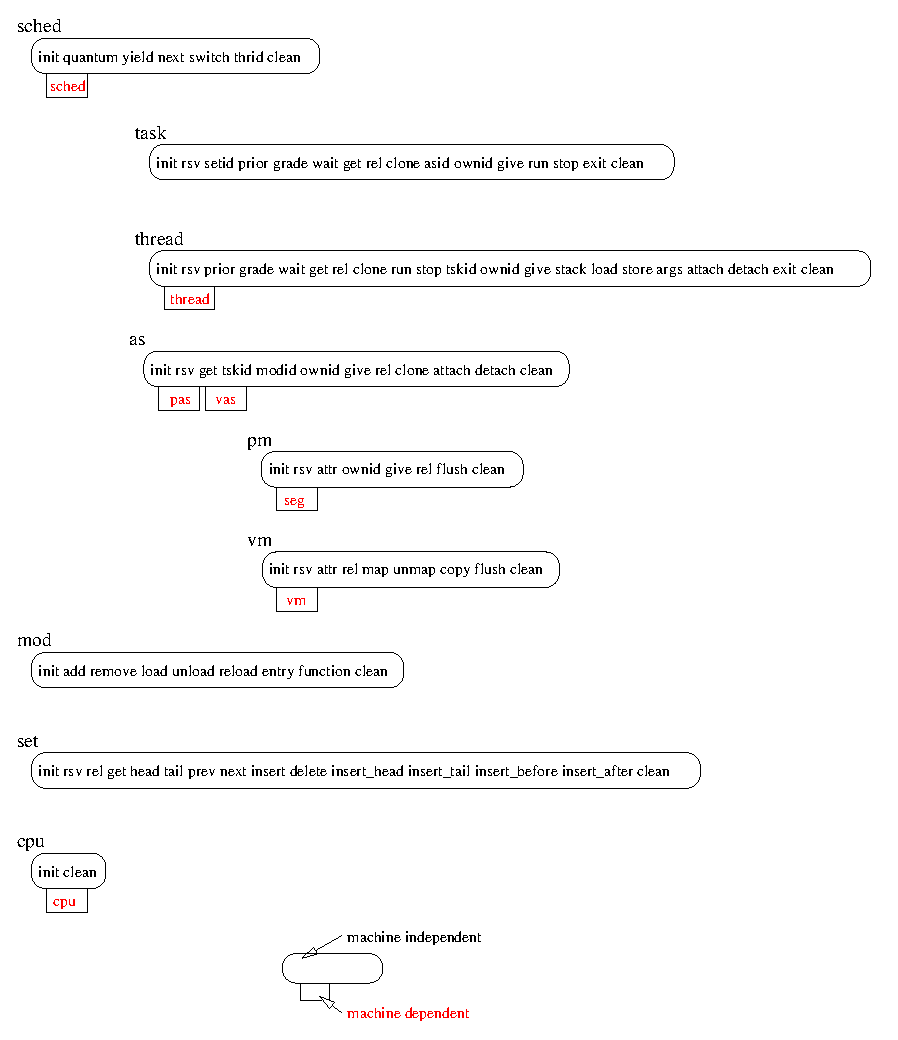
\includegraphics{figures/interfaces.eps}}
\end{figure}

\section{Bonus}

\paragraph{}

Voici les bonus pour ce projet

\subsection{Cpu detection}

\paragraph{}

Comme le titre l'indique, le but de ce bonus est de d\'etecter et r\'ecup\'erer
toutes les informations relatives au processeur: mod\`ele, puissance etc..

\paragraph{}

Lors de l'appel \`a l'initialisation du CPU, dans la fonction
\textbf{cpu\_init}(), il vous sera demand\'e d'afficher les informations
recolt\'ees.

\subsection{Parser}

\paragraph{}

Un bonus pour les personnes qui auraient ou auront effectu\'ees le bonus
du fichier de configuration. Le but cette fois ci \'etant simplement
d'int\'egrer un parser dans le gestionnaire de modules pour que celui-ci
prenne en compte le fichier de configuration lors du lancement des
services fondamentaux.

\paragraph{}

Ainsi c'est ce fichier de configuration qui indiquera au gestionnaire de
modules le nom du module, sa classe, sa priorit\'e par d\'efaut, son
comportement, son nombre de pages de pile mais \'egalement les arguments
\`a lui passer au lancement.

\subsection{Ensembles}

\paragraph{}

Le dernier bonus consiste \`a d\'evelopper des types d'ensembles
suppl\'ementaires comme par exemple: SET\_TYPE\_BTREE, SET\_TYPE\_BSTREE,
SET\_TYPE\_BPTREE etc.. mais \'egalement une interface si n\'ecessaire.

\section{Bibliographie}

\paragraph{}

Voici la bibliographie de k4.

\subsection{Ensembles}

\paragraph{}

Voici quelques liens qui pourront vous \'eclairer si vous d\'esirez
faire des templates en C.

\begin{itemize}
\item /usr/include/sys/queue.h
\item http://www.lse.epita.fr/bpt.php
\end{itemize}

\subsection{T\^aches}

\paragraph{}

\begin{itemize}
\item IA-32 Intel Architecture Software Developer's Manual Volume 3:
      System Programming Guide - Chapter 6 Task Management.
\end{itemize}

\end{document}